\documentclass{article}

% if you need to pass options to natbib, use, e.g.:
%     \PassOptionsToPackage{numbers, compress}{natbib}
% before loading neurips_2021

% ready for submission
\usepackage[preprint]{neurips_2021}

% to compile a preprint version, e.g., for submission to arXiv, add add the
% [preprint] option:
%     \usepackage[preprint]{neurips_2021}

% to compile a camera-ready version, add the [final] option, e.g.:
%     \usepackage[final]{neurips_2021}

% to avoid loading the natbib package, add option nonatbib:
%    \usepackage[nonatbib]{neurips_2021}

\usepackage[utf8]{inputenc} % allow utf-8 input
\usepackage[T1]{fontenc}    % use 8-bit T1 fonts
\usepackage[colorlinks=true]{hyperref}       % hyperlinks
\usepackage{url}            % simple URL typesetting
\usepackage{booktabs}       % professional-quality tables
\usepackage{amsfonts}       % blackboard math symbols
\usepackage{nicefrac}       % compact symbols for 1/2, etc.
\usepackage{microtype}      % microtypography
\usepackage{xcolor}         % colors
\usepackage[pdftex]{graphicx}
\usepackage{caption}
\usepackage{comment}


\title{Semantic analysis of German parliament speeches}

% The \author macro works with any number of authors. There are two commands
% used to separate the names and addresses of multiple authors: \And and \AND.
%
% Using \And between authors leaves it to LaTeX to determine where to break the
% lines. Using \AND forces a line break at that point. So, if LaTeX puts 3 of 4
% authors names on the first line, and the last on the second line, try using
% \AND instead of \And before the third author name.

\author{%
  Emanuel Fuchs\\
  Matrikelnummer xxxxxxx\\
  \texttt{emanuel-fuchs@t-online.de} \\
  \And
  Arthur Jaques\\
  Matrikelnummer xxxxxxx\\
  \texttt{arthur.jaques@live.com} \\
}

\begin{document}

\maketitle


\begin{abstract}
  This paper performs a semantic analysis of transcribed speeches in the German parliament.
  Latent Dirichlet Allocation and sentiment analysis are used to provide information about temporal shifts of topic shares and the different emphases and sentiments of parties on the extracted topics. 
\end{abstract}


\section{Introduction}
This paper describes a semantic analysis of transcribed speeches in the German parliament. 
We first extract speech topics and analyze their temporal evolution.
We then show that the credibility of the extraction by plotting the mean party topics and showing that the picture drawn is coherent to an intuitive view of the parties' differences.
Since speech topics do not explain the positions of the parties regarding them, we extract sentiments.
We finally show how non-governing parties gave on average more negative speeches across topics.


\section{Methods}
We download the texts of the Bundestag speeches from 24 October 2017 to 7 September 2021 using the OpenParliament \cite{OpenParliamentTV} API.
We discard speeches not attributed to any of the major parliament factions (\textit{SPD}, \textit{FDP}, \textit{CDU/CSU}, \textit{Bündnis 90/Die Grünen}, \textit{AfD}, \textit{Die Linke}).
We remove ``formalities'' (such as salutations) using regular expressions.
The resulting dataset contains 8,470 speeches
\footnote{2,101 \textit{CDU/CSU}, 1,547 \textit{SPD}, 1,285 \textit{AfD}, 1,188 \textit{Bündnis 90/Die Grünen}, 1,186 FDF, 1,163 \textit{Die Linke}.}.
207 different dates are present, and all parties held speeches in at least 91\% of them
\footnote{203 CDU, 195 \textit{SPD}, 198 \textit{AfD}, 193 \textit{Bündnis 90/Die Grünen}, 190 \textit{Die Linke}, 189 \textit{FDP}}.

For topic extraction, we use Scikit-learn's \cite{Scikit-learn} implementation of Latent Dirichlet Allocation, trained on the whole dataset.
The texts are stemmed using Nltk's \cite{Nltk} Snowball German Stemmer and vectorized using the bag-of-words approach with word counts.
We analyze the words having the highest weights for each topic and named the topics accordingly.
We optimize the parameters for vectorization and topic extraction to obtain interpretable results (a subjective criterion).
This results in keeping only words that appear in at least 20 speeches and at most 30\% of them for vectorization, and extracting 9 topics.
To plot the average party topic distributions, we reduce the data to 2 dimensions using Principal Component Analysis.

We extract sentiments using the Python package germansentiment \cite{Germansentiment}, which applies the Bert architecture trained on German texts.
We use p-value testing with a binomial assumption for the distribution of negative sentiments to test for asymmetrical differences between parties in the proportion of negative speeches.

\section{Results}
The topics extracted from the speeches dataset and the name that was assigned to them are summarized in Table~\ref{topics_table}.
\begin{table}
  \captionsetup{width=0.9\linewidth}
  \caption{Extracted topics}
  \label{topics_table}
  \centering
  \begin{tabular}{p{0.02\linewidth} | p{0.2\linewidth} | p{0.78\linewidth}}
    \toprule
    \# & Assigned name & Strongest predictors \\
    \midrule
    1 & International & europa; deutsch; russland; staat; gemeinsam; international; eu; menschenrecht; welt; turkei. \\
    2 & Military & soldat; einsatz; bundeswehr; mandat; soldatinn; mission; afghanistan; unterstutz; mali; militar. \\
    3 & EU/Economy & europa; euro; eu; unternehm; milliard; deutsch; prozent; union; geld; wirtschaft. \\
    4 & Social & kind; euro; famili; prozent; arbeit; sozial; 000; rent; miet; hoh. \\
    5 & Decisions/Law & gesetzentwurf; bundestag; glaub; fall; thema; hatt; word; entscheid; punkt; regel. \\
    6 & Democracy/Freedom & emokrati; leb; gesellschaft; freiheit; grundgesetz; staat; gewalt; deutsch; demokrat; wer. \\
    7 & German History & deutsch; wer; ost; geschicht; stiftung; abstimm; 19; opf; stimmt; bitt. \\
    8 & Ecology & klimaschutz; co; energi; prozent; erneuerbar; bau; ziel; verbrauch; energiew; wirtschaft. \\
    9 & Health/Pandemic & pandemi; schul; unternehm; arbeit; stark; digital; bass; bereich; massnahm; wirtschaft. \\
    \bottomrule
  \end{tabular}
\end{table}

\paragraph{Topics evolution over time}
An overview of the evolution of topics in the speeches is shown in Figure~\ref{stacked_area_plot}.
Notice the increased weights of both `Health/Pandemic' and `Decisions/Law' from the start of 2020 on, with the Covid 19 outbreak and consequent discussions about effective policy to tackle it.
An analysis of single topics such as the one done in Figure~\ref{social_topic_plot} for the `Social' topic allows to examine the relative frequency of a topic over time. 
For example there is an obvious increase in social speeches in the second half of 2018, which can be attributed to discussions about the \href{https://dserver.bundestag.de/btd/19/054/1905412.pdf}{statutory pension insurance} and the so-called \href{https://dserver.bundestag.de/btd/19/047/1904725.pdf}{Participation Opportunities Act}. 
The \href{https://dserver.bundestag.de/btd/19/075/1907504.pdf}{Strong Families Act} passed at the beginning of 2019 may also have contributed to the rise of the topic \cite{Bundestag2018}\cite{Bundestag2019}.

\begin{figure}
  \centering
  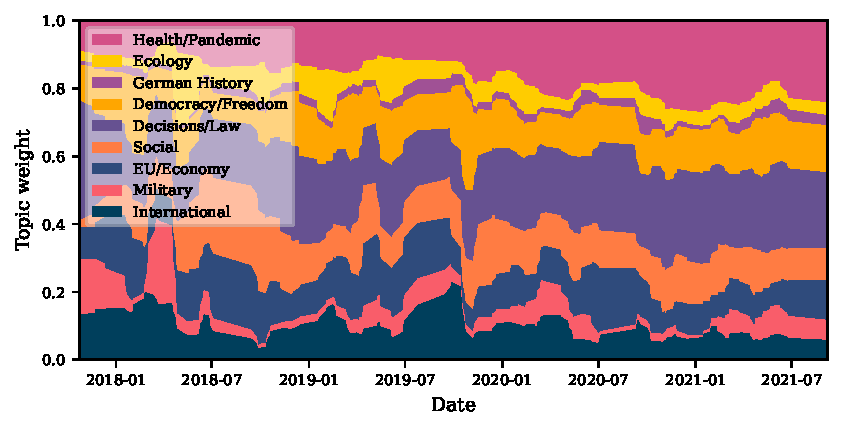
\includegraphics[width=0.9\linewidth]{images/stacked_area_plot.pdf}
  \captionsetup{width=0.9\linewidth}
  \caption{
    Average weight of topics discussed in the Bundestag (with Gaussian smoothing) between October 2017 and September 2021.
    %The topics and topic weights are extracted using Latent Dirichlet Allocation Todo(check).
  }
  \label{stacked_area_plot}
\end{figure}

\begin{figure}
  \centering
  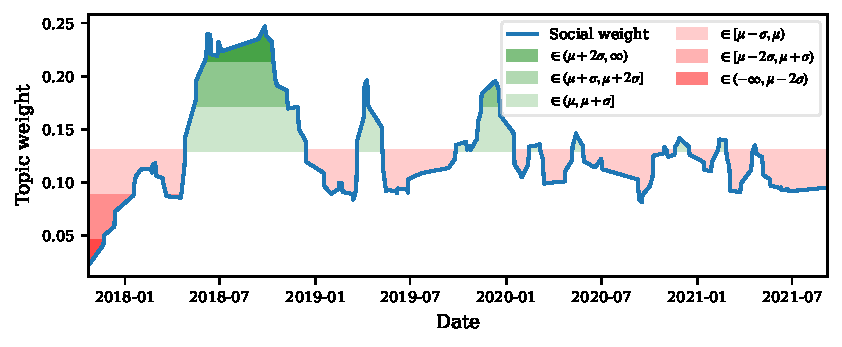
\includegraphics[width=0.9\linewidth]{images/Social.pdf}
  \captionsetup{width=0.9\linewidth}
  \caption{
    Average weight of the `Social' topic in the Bundestag speeches (with Gaussian smoothing) between October 2017 and September 2021.
  }
  \label{social_topic_plot}
\end{figure}


\paragraph{Party topics differences}
In Figure~\ref{pca_plot} we show the results of 2-dimensional Principal Component Analysis on the average topic weights for each party.
The results show the parties more or less sorted on the left-right axis along the second principal component.
Furthermore, it shows the two parties that are considered more `extremist' (`\textit{Die Linke}' and `\textit{AfD}') significantly distant from the other parties.
We notice how the new \textit{Ampel Koalition}, that wasn't governing at the time, was already closer together than the governing \textit{Schwarz-rote Koalition}.

\begin{figure}
  \centering
  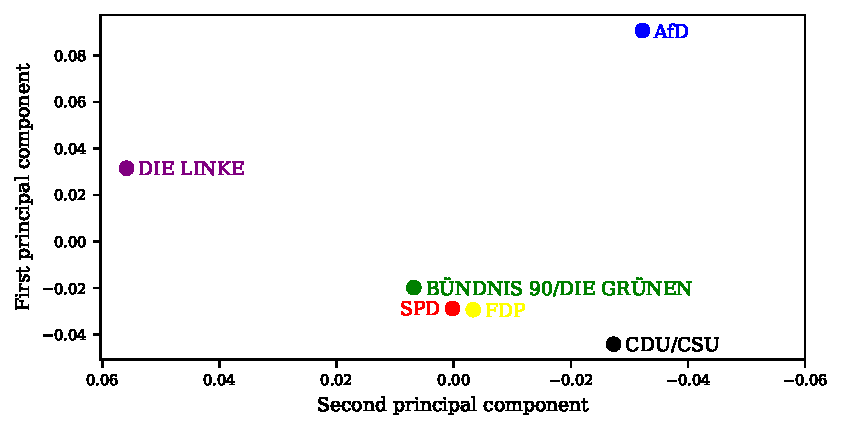
\includegraphics[width=0.9\linewidth]{images/pca.pdf}
  \captionsetup{width=0.9\linewidth}
  \caption{
    Principal Component Analysis on average topics per party.
  }
  \label{pca_plot}
\end{figure}


\paragraph{Sentiment analysis}
The extraction of sentiments from the speeches yielded in total 7,293 neutral speeches, 1,179 negative speeches, and 13 positive speeches.
Figure~\ref{sentiments_plot} shows the average sentiment by party and topic.
The plot suggests more negative speeches of non-governing parties (with `\textit{FDP}' as an exception).
We perform a p-value test for significant differences between the average proportion of negative speeches over all parties and single parties
\footnote{We concentrate the analysis on negative sentiments, since very few positive sentiments are found.}.
We assume a binomial distribution of the amount of negative speeches, and use beta-distributed priors.
We obtain p-values for the asymmetrical differences between the binomial negative speech probability of the whole set of speeches and the speeches of specific parties.
Using a threshold $\alpha$ of $0.05$ with Bonferroni correction for multiple testing
\footnote{2 asymmetrical tests per party and 6 parties yield 12 hypotheses, and a corrected $\alpha=0.004$}
we refute the null hypotheses that both `\textit{SPD}' and `CDU' have a bigger or equal probability of a negative speech than the Bundestag's mean,
and that `\textit{Bündnis 90/Die Grünen}', `\textit{AfD}', and `\textit{Die Linke}' have smaller or equal probability of a negative speech than the Bundestag's mean.
We did not obtain significant results for both asymmetrical tests in the case of `\textit{FDP}'.
These results are coherent with the hypothesis that non-governing parties tend to hold more negative speeches.

\begin{figure}
  \centering
  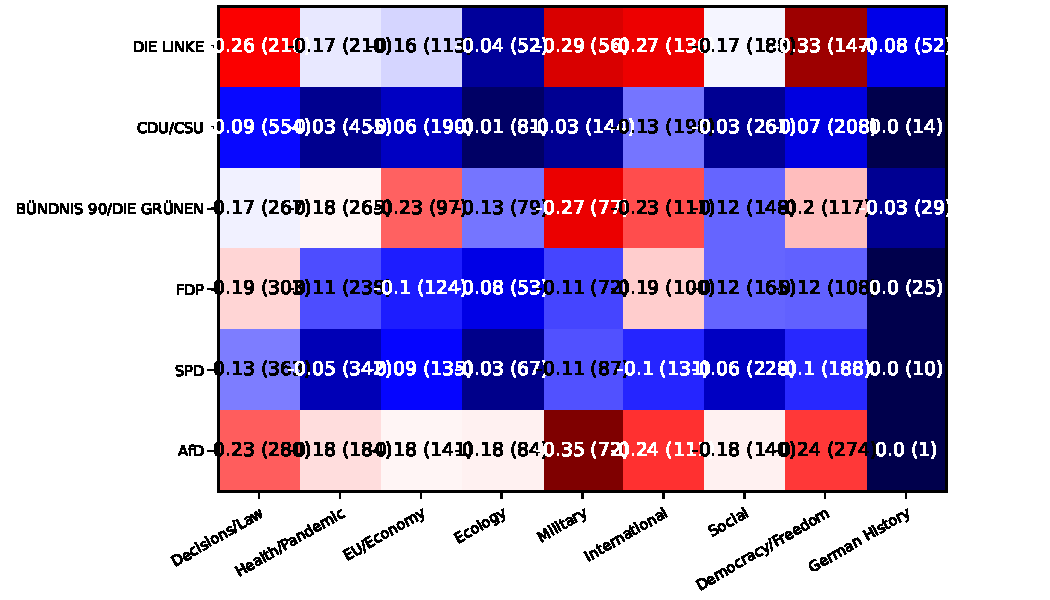
\includegraphics[width=0.9\linewidth]{images/sentiments_confusion.pdf}
  \captionsetup{width=0.9\linewidth}
  \caption{
    Average sentiment (from -1, fully negative, to +1, fully positive) by party and topic, extracted using the Python package germansentiment \cite{Germansentiment}.
    The number in brackets indicates the number of speeches the mean is constructed from, to give an idea of the significance of the number (low for example for `History' topic).
    Each speech is assigned to a single topic (the one with the highest weight).
  }
  \label{sentiments_plot}
\end{figure}


\section{Discussion and conclusion}

Our methodology entails some limitations that suggest caution when interpreting the results. 
In the used dataset some speeches are missing.
However, since the data loss is due to technical reasons, we might assume that the effect is random and the available data provide a good representation.
Furthermore, the data cover a short period of 4 years, which leads to a high influence of individual fluctuations.
Besides the usual limitations of the used methods, in topic extraction the best parameters and topics names were selected subjectively.
When implementing p-value testing, the issue arises that the party data is contained in the aggregate data as well.
This however makes the distributions more similar and increases the p-value, making it more difficult to show significant results.
Thus, this procedure decreases the number of significant results and does not invalidate our results.

Despite these limitations, the methodology used is promising.
Meaningful results were obtained and topics such as the Health/Pandemic behave as expected. 
In addition, the created figures give good information about the temporal behavior and the differences between parties.
More data is needed to test for party-sentiment-topic correlations, analyze the topics' evolution over time, and further test the hypothesis that non-governing parties hold more negative speeches (for this, we would need to test over different governing coalitions).

\begin{comment}
  Limitations:
  \begin{itemize}
    \item Data: incomplete data, aggressive procedure to get data, reliance of data
    \item Visualization: smoothing (free parameters), short time frame, topics dictated by agenda
    \item Topic extraction: free parameters, subjectivity of chosen topic names
    \item Sentiment analysis: black-box model
    \item p-value testing: correlated hypotheses, unbalanced data, data contained in both sets
  \end{itemize}
  
\end{comment}

\bibliographystyle{plain}
\bibliography{bibliography}

\end{document}
